\documentclass[10pt]{article}
\usepackage[margin=0.7in]{geometry}
\usepackage{graphicx,booktabs,amsmath,caption,array}
\graphicspath{{../figures/}{figures/}}
\captionsetup{font=small,labelfont=bf,skip=3pt}
\setlength{\parindent}{0pt}\setlength{\parskip}{3pt}
\renewcommand{\arraystretch}{1.05}
\title{\vspace{-1.2cm}\textbf{An independent external evaluation of the Aiki-Sol public beta\\ for protein solubility prediction}\vspace{-0.3cm}}
\newcommand{\authorname}{Aaron Ezekiel}
\author{\small \authorname, undergraduate, UC Berkeley\\ \small Independent evaluation, prepared for Aikium, Inc.}
\date{\small October 2026}
\begin{document}\maketitle\vspace{-0.9cm}
\begin{abstract}\small\noindent
We independently tested the public beta of Aiki-Sol, an ESM-2-based predictor of \emph{E.~coli} soluble expression, on 500 sequences (250 soluble, 250 insoluble) sampled from the UESolDS independent test split. The pre-specified primary metric, AUROC of the protocol-agnostic marginal output, was \textbf{0.858} (95\% bootstrap CI 0.823--0.891), versus 0.608 for a five-feature logistic regression and 0.506 for the published SWI index. \textbf{Leakage cannot be ruled out}: 64.8\% of the evaluated sequences are exact matches to Aiki-Sol's released training pool, so 0.858 is an upper bound on performance for novel proteins; on the 176 non-matching sequences AUROC was 0.741 (0.668--0.807). The marginal output was reasonably calibrated (Brier 0.156). One benchmark and one mixed-protocol label set were used; everything beyond the primary metric is exploratory.
\end{abstract}
\section*{1\quad Introduction}
In nanobody (VHH) discovery, candidates must be expressed in a bacterial host before they can be characterised, so sequence-based filters that flag poorly soluble candidates before synthesis could save cost and time. Aiki-Sol (Aikium; bioRxiv 10.64898/2026.05.14.725067) predicts the probability that a sequence stays soluble under each of five centrifugation protocols plus a protocol-agnostic ``marginal'' output. Its public beta, hosted API, source code and weights are openly available.
An outside check is worthwhile for a new tool whose preprint is not yet peer reviewed, especially because the standard solubility benchmarks largely derive from the same structural-genomics sources used for training. This report is written as a curious external user's validation, not a review: it states what worked as prominently as what did not.
\section*{2\quad Methods}
\textbf{Access and gates.} The advertised \texttt{pip install aikisol} fails (no PyPI package); I ran the unmodified GitHub source (commit d8fcbf86) with the Zenodo canonical checkpoint on CPU. Docker was not tried. The hosted REST API and the local package agree to $\le 2\times10^{-6}$ on all outputs (40 sequences), so bulk scoring ran locally; the API was used for gates and probes (126 of 1,500 permitted requests). \emph{Gate 1a (my pipeline)}: SWI, a published predictor, on the UESolDS test split (4,000 sequences, 2,000/2,000 as published) reproduced the published AUC 0.5597 exactly (mine 0.5597; accuracy 0.5423, sensitivity 0.7905, specificity 0.2940 vs 0.2938). SoluProt (needs TMHMM, USEARCH) and NetSolP (5.6 GB) were not run. \emph{Gate 1b (Aiki-Sol direction)}: 20 hand-picked soluble and 20 inclusion-body controls were nominally ordered correctly (marginal 0.907 vs 0.880) but not separated (AUC 0.475, CI 0.29--0.66): many mature, disulfide-rich cytokines score $>0.99$. Calling and parsing were verified as correct (echoed sequences identical, API = local). A supplementary check added after this result, on 100 labelled train-split sequences, confirmed direction: AUC 0.752 (0.650--0.839), soluble 0.583 vs insoluble 0.282 (one-sided $p<0.001$).\\
\textbf{Data and protocol match.} Evaluation set: 250+250 sequences drawn with seed 20261028 from the UESolDS independent test split (Zhang et al., 2024; labels from structural-genomics pipelines and PDB deposition; $\le$25\% identity to the training sets of seven earlier predictors); CPU-only scoring limited $N$. No single centrifugation regime matches these mixed labels, so \emph{before scoring} I fixed the \textbf{marginal output} (documented as the choice for unspecified protocols) as primary; the five regimes are secondary. A protocol mismatch is therefore a limitation of my design, not a flaw of the tool. The primary metric (AUROC with 2,000-resample percentile CI) and all analysis choices were hashed before any Aiki-Sol score was obtained.\\
\textbf{Baselines and statistics.} Logistic regression on length, GRAVY, net charge at pH~7, charged fraction and aromatic fraction, fit on the benchmark's train split (70,029 sequences; a provisional fit during a network outage gave 0.645, same conclusions); SWI; majority class. Differences are paired bootstraps; a winner is named only if the interval excludes zero. Leakage audit: exact MD5 match (raw, Met-added or Met-stripped) against the released 147,574-sequence training list.
\section*{3\quad Results}
\textbf{Primary.} Aiki-Sol marginal AUROC was \textbf{0.858 (0.823--0.891)}, well above the logistic-regression floor (paired difference $+0.251$, CI $+0.194$ to $+0.308$) and SWI ($+0.353$, $+0.295$ to $+0.414$; Table~1, Fig.~1). \emph{Secondary (exploratory):} AUPRC 0.868; at threshold 0.5 accuracy 0.770, sensitivity 0.744, specificity 0.796, MCC 0.541 (the Youden-optimal threshold, 0.465, is chosen on the same data and gives MCC 0.560, optimistic). The five regime outputs scored 0.820--0.854 and none beat the marginal output; the cell-free (PURE) output was lowest, 0.820 (0.780--0.855), with overlapping intervals, so I draw no protocol-sensitivity conclusion. AUROC by length tercile was 0.851, 0.890 and 0.825 (overlapping CIs), with no marked length effect (Spearman score--length $-0.22$).
\begin{table}[h]\centering\small
\begin{tabular}{lccccc}\toprule
Model & AUROC (95\% CI) & AUPRC & MCC & Sens. & Spec.\\\midrule
\textbf{Aiki-Sol, marginal output} & \textbf{0.858} (0.823--0.891) & 0.868 & 0.541 & 0.744 & 0.796\\
Logistic regression, 5 features & 0.608 (0.557--0.654) & 0.573 & 0.189 & 0.964 & 0.144\\
SWI (published) & 0.506 (0.453--0.555) & 0.490 & 0.086 & 0.772 & 0.304\\
Majority class & 0.500 & -- & 0 & -- & --\\\bottomrule
\end{tabular}
\caption{Primary result (AUROC, bold) and secondary metrics on $N{=}500$ (250/250); thresholds at 0.5. Aiki-Sol's AUROC interval does not overlap either baseline's.}
\end{table}
\begin{figure}[h]\centering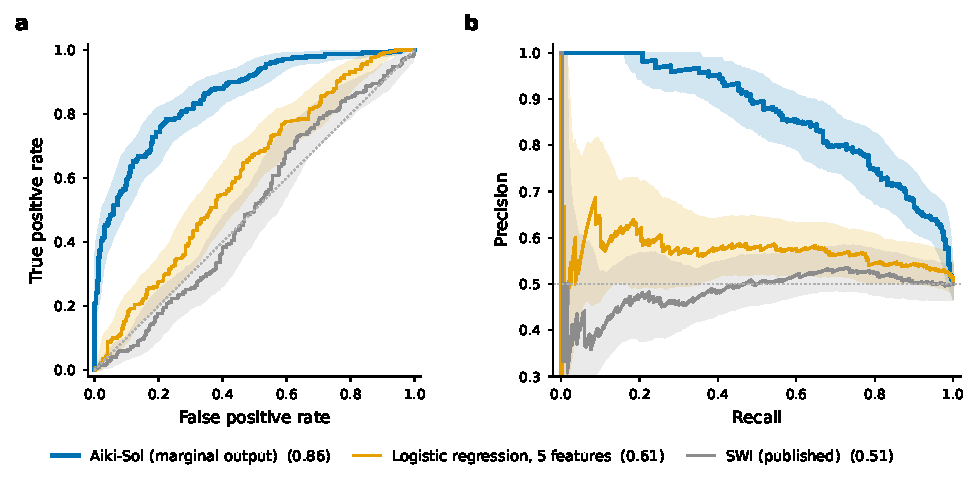
\includegraphics[width=0.93\linewidth]{fig1_roc_pr.pdf}
\caption{ROC (a) and precision--recall (b) curves on 500 UESolDS test sequences (250 soluble); legend gives AUROC. Bands: 95\% pointwise percentile intervals over 1,000 bootstrap resamples. Dotted lines: chance. Aiki-Sol's band does not overlap the baselines' over most of the range.}
\end{figure}
\textbf{Leakage and confounding (central to interpretation).} 324/500 evaluated sequences (64.8\%; 2,594/4,000 in the full split) are exact matches to the released training list. AUROC was 0.912 (0.880--0.940) on those and 0.741 (0.668--0.807) on the 176 non-matches (logistic regression 0.638 and 0.519). Exact matches mean the sequence was seen in training, not that its label was identical, and the two strata differ in source mix, so the gap is suggestive rather than a clean memorisation estimate. Near-identical homologues may remain among the non-matches. Separately, labels track the contributing consortium: all 113 PDB-derived sequences are soluble, and consortium identity alone (in-sample) gives AUROC 0.825. Within consortia Aiki-Sol still ranks well (JCSG, $n{=}98$: 0.732, 0.628--0.827; MCSG, $n{=}94$: 0.890, 0.816--0.946), so the signal is not only source.\\
\textbf{Calibration (claim tested directly).} The marginal output was reasonably calibrated on this balanced set: Brier 0.156 (0.135--0.178) versus 0.254 for logistic regression, ECE 0.044 (0.036--0.091), intercept $+0.03$, slope 0.85 (mild overconfidence); mean prediction 0.492 against 0.500 observed (Fig.~2). Regime-specific outputs were less calibrated here (ECE 0.055--0.132; PURE 0.250, mean 0.75), as expected when labels do not follow those protocols; this does not test their per-protocol claim.\\
\begin{minipage}[t]{0.34\linewidth}\vspace{0pt}\centering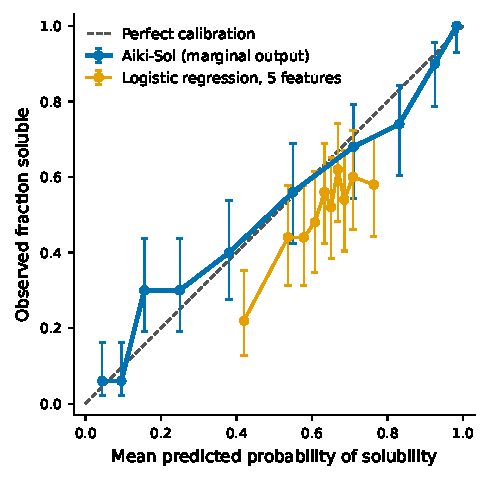
\includegraphics[width=\linewidth]{fig2_calibration.pdf}
\captionof{figure}{Reliability of predicted probability (equal-frequency deciles, $n{\approx}50$; 95\% Wilson intervals), Aiki-Sol marginal vs.\ logistic regression.}\end{minipage}\hfill
\begin{minipage}[t]{0.63\linewidth}\vspace{0pt}\small
\textbf{Probes (exploratory; $n{=}24$ sequences, length-matched controls).} \emph{Tags:} the real tag's score shift is compared with a same-leader control (His6 replaced by a random non-His 6-mer; SUMO replaced by a scrambled copy). A composition-matched His6 control is impossible (a shuffled HHHHHH is HHHHHH). \emph{N-terminal His6} (pET-28a-style leader): mean $|\Delta|$ 0.100 vs control 0.134 (difference $-0.033$, CI $-0.074$ to $+0.002$); \emph{C-terminal His6}: 0.028 vs 0.026 ($+0.003$, $-0.010$ to $+0.017$). Tags are detected in 24/24 and stripped, leaving a 2--3 residue linker scar. I found \emph{no evidence of incomplete His6 stripping}. \emph{SUMO} (not among the documented stripped tags) raised P(soluble) by $+0.44$ vs $-0.15$ for the scramble (difference in $|\Delta|$ $+0.265$, $+0.076$ to $+0.445$): expected from the documentation, but a user scoring a SUMO fusion would see an inflated score. A 6-sequence API replication matched local scores ($\le 7\times10^{-6}$).
\end{minipage}\\[3pt]
\textbf{Determinism and robustness.} Repeat scoring was identical (local: max difference 0; API, 10 sequences $\times$2: identical; alone-vs-batched $7\times10^{-7}$). An empty input returns a clear HTTP 400. Otherwise the tool accepts essentially any input without complaint: X/B/Z/U and lowercase are handled, 2--5 residue peptides score $\approx$0.99, and a 100-residue poly-His normalises to an empty sequence yet still receives a score (0.248). I found no documented claim of input validation, so these are observations, not defects. Two SUMO constructs returned HTTP 500; they are exactly the two for which the local normaliser leaves a His6 in the sequence, matching the documented retained-tag preflight, which appears to surface as an unexplained 500.
\section*{4\quad Discussion}
\textbf{What works.} Aiki-Sol clearly beats simple baselines on this benchmark, is deterministic, fast (about 1.3\,s per API call), reasonably calibrated on the marginal output, and unusually auditable: weights, training list and splits are public, and the hosted tool equals the released checkpoint. \textbf{Limitations.} (i) Leakage: 65\% exact overlap makes 0.858 an upper bound; 0.741 on non-matches is more representative but still not leakage-proof. (ii) One benchmark, $N{=}500$, intervals of roughly $\pm$0.03 (primary) to $\pm$0.07 (strata). (iii) The label--consortium confound and mixed protocols; the marginal output was chosen because no regime fits, and no claim about per-protocol accuracy is possible. (iv) Five regimes were examined, so any single regime gap is uncorrected for multiplicity. (v) Weak controls in Gate 1b (resolved by the supplementary check); a logistic-regression baseline trained in-distribution has an advantage over a zero-shot tool; only SWI was re-run as a published predictor. (vi) The nanobody subset was not done: no public labelled VHH solubility set was found and Aikium's nanobody cohorts are not released. The probes are small. \textbf{Suggestions.} (1) Publish the \texttt{aikisol} package to PyPI or correct the README. (2) Document that SUMO and other large fusions are not stripped, and return a descriptive 4xx instead of HTTP 500 when the retained-tag check fails. (3) Release or point to a post-training-cutoff held-out set and report performance on sequences below an identity threshold to the training list.
\vspace{2pt}{\footnotesize\textbf{References.} Aikium. Aiki-Sol, bioRxiv 10.64898/2026.05.14.725067; weights/data Zenodo 10.5281/zenodo.20151817. Zhang X.\ et al.\ PLM\_Sol, Brief.\ Bioinform.\ 25(5):bbae404 (2024). Bhandari B.K., Gardner P.P., Lim C.S.\ SWI, Bioinformatics, 10.1093/bioinformatics/btaa578 (2020). Hon J.\ et al.\ SoluProt, Bioinformatics 37(1) (2021). Thumuluri V.\ et al.\ NetSolP, Bioinformatics 38(4):941 (2022).}
\end{document}
